%\documentclass[12pt,aspectratio=169]{beamer}
\documentclass[12pt,english]{beamer}
%\documentclass[20pt,handout]{beamer}

%\usetheme{default}
%\usetheme{AnnArbor}
%\usetheme{Antibes}
%\usetheme{Bergen}
%\usetheme{Berkeley}
%\usetheme{Berlin}
\usetheme{Boadilla}
%\usetheme{CambridgeUS}
%\usetheme{Copenhagen}
%\usetheme{Darmstadt}
%\usetheme{Dresden}
%\usetheme{Frankfurt}
%\usetheme{Goettingen}
%\usetheme{Hannover}
%\usetheme{Ilmenau}
%\usetheme{JuanLesPins}
%\usetheme{Luebeck}
%\usetheme{Madrid}
%\usetheme{Malmoe}
%\usetheme{Marburg}
%\usetheme{Montpellier}
%\usetheme{PaloAlto}
%\usetheme{Pittsburgh}
%\usetheme{Rochester}
%\usetheme{Singapore}
%\usetheme{Szeged}
%\usetheme{Warsaw}

\usepackage{graphicx}
\usepackage[ngerman,english]{babel}
\usepackage[T1]{fontenc}
\usepackage[utf8]{inputenc}
\usepackage{tikz}
\setbeamertemplate{footline}[frame number]
\usepackage{textcomp}
\usepackage{hyperref}
\usepackage[style=american]{csquotes}

\newcommand{\cc}[1]{\includegraphics[height=2cm]{img/#1.pdf}}
\usepackage{ifthen}
\newcommand{\license}[2][]{\\#2\ifthenelse{\equal{#1}{}}{}{\\\scriptsize\url{#1}}}

%mainly used for maxyms slides
\newcommand {\framedgraphic}[1] {
    \begin{frame}
        \begin{center}
            \includegraphics[width=\textwidth,height=0.8\textheight,keepaspectratio]{#1}
        \end{center}
    \end{frame}
}

\pgfdeclareimage[height=0.8cm]{logo}{./BitcoinSign.pdf} 
\pgfdeclareimage[height=0.8cm]{torlogo}{./tor-onion.pdf} 
\pgfdeclareimage[height=0.8cm]{stellarlogo}{./stellar.png} 


\pgfdeclarelayer{foreground}
\pgfsetlayers{main,foreground}
%\logo{\pgfputat{\pgfxy(-1,0)}{\pgfbox[center,base]{\pgfuseimage{logo}}}}

\title{Special Purposes Seminar \\ \textbf{Freedom on the Internet} }
\author{\small David\,(s72838), Maxym\,(s72810), Wolf\,(s72785)  }
\date{21.05.2015, Dresden University of Applied Sciences }

\begin{document}
\maketitle

\section{Introduction}
\subsection{}

\begin{frame}
	\frametitle{What is it about?}
		\begin{center}
			
\includegraphics[height=0.5\textheight]{./img/logo-transp.png} \\
			\mbox{\textbf{if you are free --- you cannot be free of risk}}
		\end{center}
\end{frame}

\begin{frame}
	\frametitle{What we are presenting}
	\begin{itemize}
		\item tor project: \textbf{t}he \textbf{o}nion \textbf{r}outing
		\item Bitcoin: peer-to-peer electronic cash
		\item Stellar.org: free and open-source exchange
	\end{itemize}
\end{frame}

\pgfdeclarelayer{foreground}
\pgfsetlayers{main,foreground}
\logo{\pgfputat{\pgfxy(-1,0)}{\pgfbox[center,base]{\pgfuseimage{torlogo}}}}

\section{tor}
\subsection{}

\framedgraphic{./img/tor_presentation/s1.png}

\framedgraphic{./img/tor_presentation/s2.png}

\framedgraphic{./img/tor_presentation/s3.png}

\framedgraphic{./img/tor_presentation/s4.png}

\framedgraphic{./img/tor_presentation/s5.png}

\framedgraphic{./img/tor_presentation/s6.png}

\framedgraphic{./img/tor_presentation/s7.png}

%~ \begin{frame}
	%~ \frametitle{ ... }
%~ 
%~ \begin{columns}[T]
    %~ \begin{column}{.3\textwidth}
    %~ \begin{block}{...}
%~ %		\includegraphics[width=1.9cm]{./img/WikipediaBinary.pdf}
    %~ \end{block}
    %~ \end{column}
    %~ \begin{column}{.7\textwidth}
     %~ \begin{block}{...}
	%~ \begin{itemize}
		%~ \item ...
	%~ \end{itemize}
    %~ \end{block}
    %~ \end{column}
  %~ \end{columns}
%~ 
%~ \end{frame}

\pgfdeclarelayer{foreground}
\pgfsetlayers{main,foreground}
\logo{\pgfputat{\pgfxy(-1,0)}{\pgfbox[center,base]{\pgfuseimage{logo}}}}

\section{Bitcoin}
\subsection{}

\begin{frame}
	\frametitle{}
\begin{columns}[T]
    \begin{column}{.3\textwidth}
    %\begin{block}{...}
		
\includegraphics[width=3.5cm]{./img/btc_presentation/pos.jpg}
    %\end{block}
    \end{column}
    \begin{column}{.5\textwidth}
     \begin{block}{advantages}
	\begin{itemize}
		\item decentralized: peer-to-peer
		\item no limiting third party
		\item low fees and init. costs
		\item encouraging ruleset
	\end{itemize}
    \end{block}
    \end{column}
  \end{columns}
\end{frame}

\begin{frame}
	\frametitle{}
	\begin{columns}[T]
    \begin{column}{.5\textwidth}
	\begin{block}{other properties}
	\begin{itemize}
		\item value created by believe/experience
		\item backed by users and services
		\item predictable mining
		\item high fungability
		\item no chargebacks
	\end{itemize}
	\end{block}
    \end{column}
    \begin{column}{.4\textwidth}
		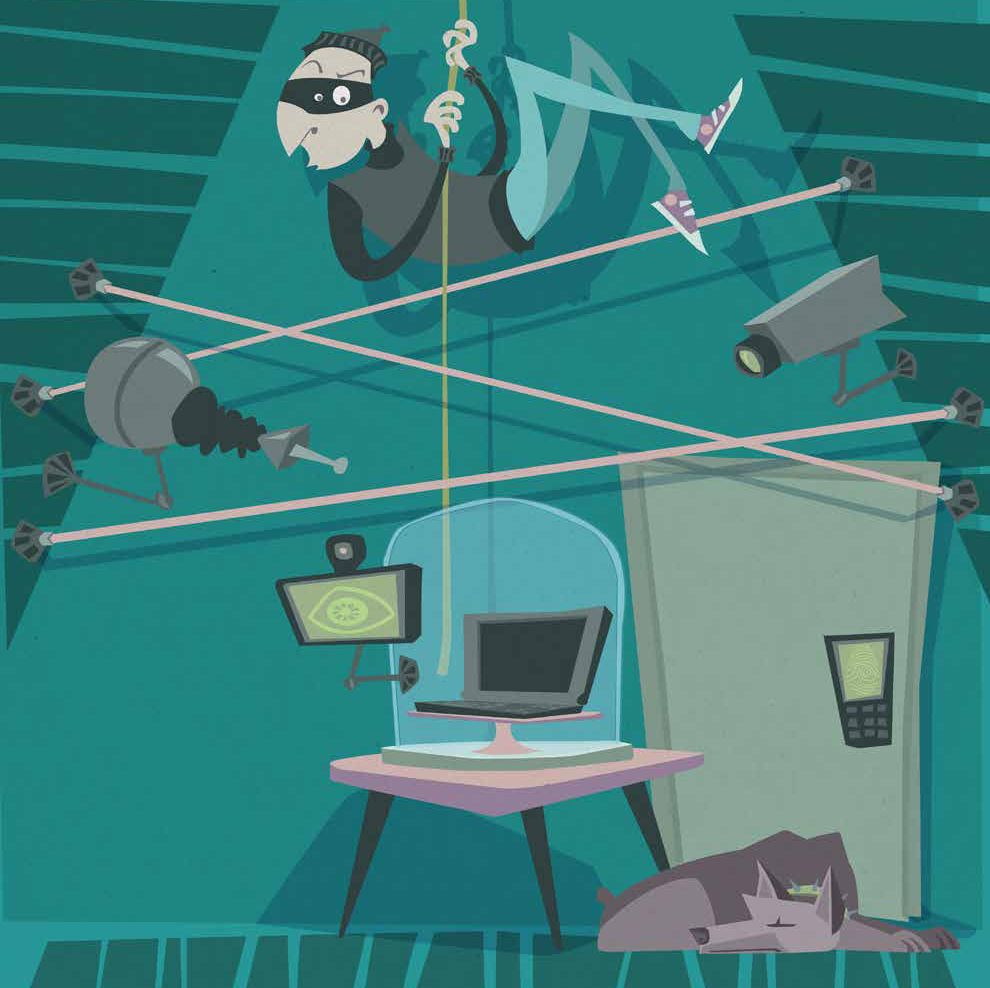
\includegraphics[width=4.5cm]{./img/btc_presentation/thief.png}
    \end{column}
  \end{columns}
\end{frame}

\begin{frame}
	\frametitle{}
	\begin{block}{some numbers}
	\begin{itemize}
		\item 10min-avg. verified transaction
		\item 2 weeks adjusting difficulty
		\item 7 tx/sec with 1MB blocks
		\item fungability 8 decimal places
		\item key space: 2\^160 = 51 dec.pl. 
		\item block halfing each 4y
	\end{itemize}
	\end{block}
\end{frame}

\begin{frame}
	\frametitle{}
  \begin{columns}[T]
    \begin{column}{.4\textwidth}
		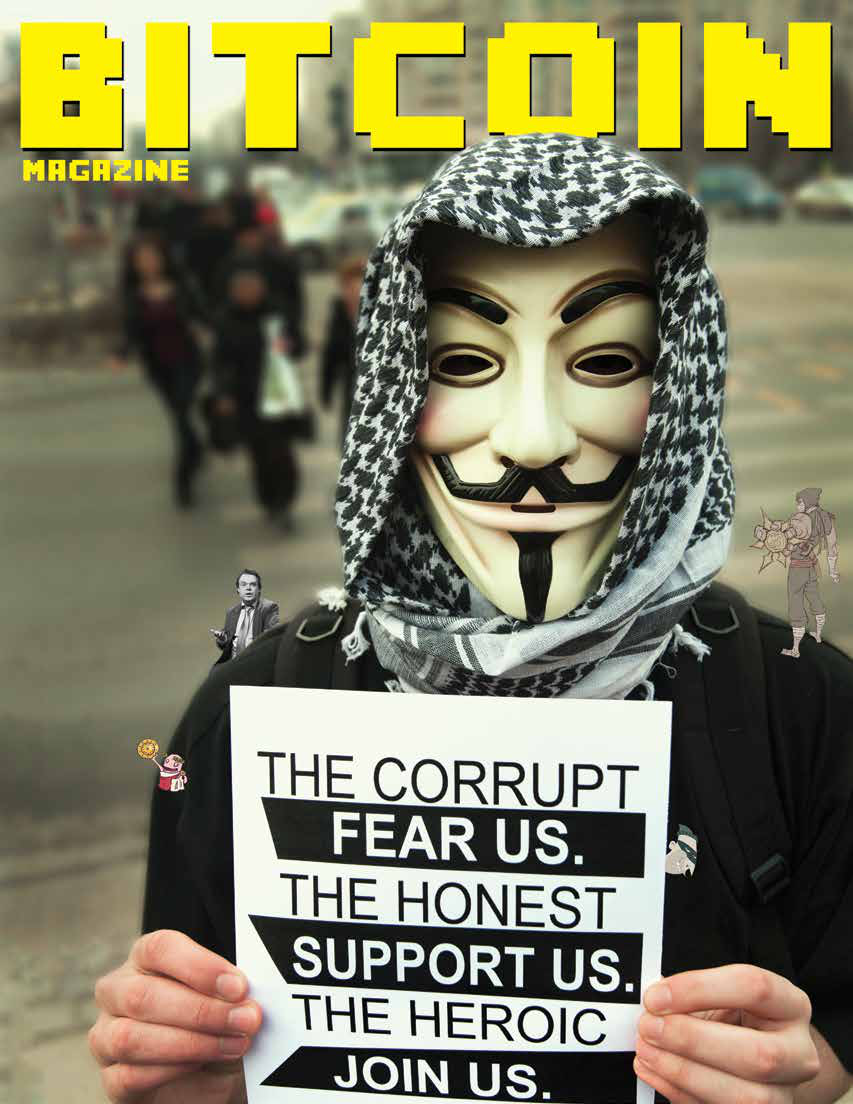
\includegraphics[width=5cm]{./img/btc_presentation/bm.png}
    \end{column}
    \begin{column}{.5\textwidth}
	\begin{block}{zero trust}
	\begin{itemize}
		\item free software, open standard
		\item address is public key
		\item money can be spent with secret key
		\item reference to source of assets
		\item responsibiliy: yours
	\end{itemize}
	\end{block}
    \end{column}
  \end{columns}
\end{frame}

\framedgraphic{./img/btc_presentation/blockchain.png}

\begin{frame}
	\frametitle{}
  \begin{columns}[T]
    \begin{column}{.4\textwidth}
	\begin{block}{mining}
	\begin{itemize}
		\item free software, open standard
		\item address is public key
		\item money can be spent with secret key
		\item reference to source of assets
		\item responsibiliy: yours
	\end{itemize}
	\end{block}
    \end{column}
    \begin{column}{.5\textwidth}
		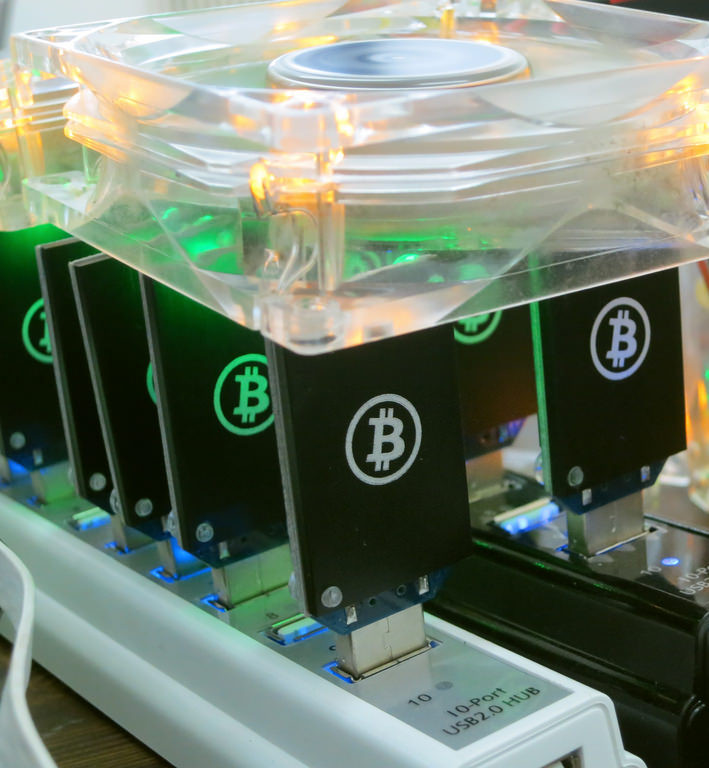
\includegraphics[width=5.5cm]{./img/btc_presentation/miner.jpg}
    \end{column}
  \end{columns}
\end{frame}


%~ \subsection{core:blockchain}
%~ 
%~ \begin{frame}
	%~ \frametitle{}
	%~ \begin{itemize}
		%~ \item all transaction on bitcoin
		%~ \item every full node has a copy
		%~ \item 
	%~ \end{itemize}
%~ \end{frame}

\pgfdeclarelayer{foreground}
\pgfsetlayers{main,foreground}
\logo{\pgfputat{\pgfxy(-1,0)}{\pgfbox[center,base]{\pgfuseimage{stellarlogo}}}}

\section{Stellar}
\subsection{}

%\begin{frame}
%	\frametitle{}
%		\includegraphics[width=1.9cm]{./img/stellar_presentation/bild.jpg}
%	\begin{itemize}
%		\item ...
%	\end{itemize}
%\end{frame}

\framedgraphic{./img/stellar_presentation/bild_1.jpg}

\framedgraphic{./img/stellar_presentation/bild_2.jpg}

\framedgraphic{./img/stellar_presentation/bild_3.jpg}

\framedgraphic{./img/stellar_presentation/bild_4.png}

\framedgraphic{./img/stellar_presentation/bild_5.jpg}

\framedgraphic{./img/stellar_presentation/bild_6.jpg}

\framedgraphic{./img/stellar_presentation/bild_7.jpg}

\framedgraphic{./img/stellar_presentation/bild_8.jpg}

\framedgraphic{./img/stellar_presentation/bild_9.jpg}

\framedgraphic{./img/stellar_presentation/bild_10.jpg}

\framedgraphic{./img/stellar_presentation/bild_11.png}

\begin{frame}
	\frametitle{Sources}
	\begin{itemize}
		\item tor:\enquote{Bild 2.} \url{http://ntrg.cs.tcd.ie/undergrad/4ba2.05/group10/}, Web.~20\,May\,2015
		\item tor:\enquote{Bild 3-5.} \url{https://www.torproject.org/about/overview.html.en}, Web.~20\,May\,2015
		\item \enquote{Learn.} Stellar. https://www.stellar.org/learn/, Web.~1\,Apr.\,2015. 
		\item bitcoin:\enquote{brainwallet.org}. Web.~20\,May\,2015
	\end{itemize}
\end{frame}

%\section{}
\subsection{one more thing}

\framedgraphic{./img/btc_presentation/jsjeopardy.png}

\end{document}
